\documentclass[final,6p,times,twocolumn]{elsarticle}
\makeatletter

\renewenvironment{abstract}{\global\setbox\absbox=\vbox\bgroup
  \hsize=\textwidth\def\baselinestretch{1}%
  \noindent\unskip\textbf{Resumen}  % <--- Edit as necessary
 \par\medskip\noindent\unskip\ignorespaces}
 {\egroup}

\def\keyword{%
  \def\sep{\unskip, }%
 \def\MSC{\@ifnextchar[{\@MSC}{\@MSC[2000]}}
  \def\@MSC[##1]{\par\leavevmode\hbox {\it ##1~MSC:\space}}%
  \def\PACS{\par\leavevmode\hbox {\it PACS:\space}}%
  \def\JEL{\par\leavevmode\hbox {\it JEL:\space}}%
  \global\setbox\keybox=\vbox\bgroup\hsize=\textwidth
  \normalsize\normalfont\def\baselinestretch{1}
  \parskip\z@
  \noindent\textit{Palabras clave: }  % <--- Edit as necessary
  \raggedright                         % Keywords are not justified.
  \ignorespaces}



\usepackage[spanish]{babel}

\def\ps@pprintTitle{%
     \let\@oddhead\@empty
     \let\@evenhead\@empty
     \def\@oddfoot{\footnotesize\itshape
        \ifx\@journal\@empty   % <--- Edit as necessary
       \else\@journal\fi\hfill\today}%
     \let\@evenfoot\@oddfoot}




\usepackage{graphicx}

\usepackage{amssymb}

\usepackage{lineno}

\usepackage{float}

%\journal{FIME}

\begin{document}

\begin{frontmatter}



\title{Comprobación de los efectos de los super esparcidores en simulación de epidemia con sistema multiagente }





\address{Universidad Autónoma de Nuevo León.}

\address{Facultad de Ingeniería Mecánica y Eléctrica.}

\author{Victor A. Oviedo }


\begin{abstract}
En este artículo se pretende observar y comprobar los efectos de los llamados super esparcidores en la simulación de epidemia con sistema multiagente, con características del virus SARS-CoV-2. La totalidad de la simulaciones son realizadas en el software libre Python \cite{Python}. 
\end{abstract}



\begin{keyword}
Epidemia \sep sistema multiagente   \sep super esparcidor.
\end{keyword}

\end{frontmatter}



%----------------------------------------------------------------------------------------------




\section{Introducción}

Este trabajo surge como continuación a la actividad \cite{VO-P6}, en el cual es una introducción a los sistemas multiagente tomando como tópico las epidemias. Se tomó la decisión de simular los efectos de los super esparcidores después de leer el artículo \cite{Cox}, en donde el autor habla sobre la decisión de: ¿A quién vacunar?, ya que la epidemia puede ser controlada con mayor eficiencia dependiendo de a quien se le aplique la vacuna. Por lo tanto, hablamos de detener el contagio con el menor número de vacunas. 


%----------------------------------------------------------------------------------------------





\section{Antecedentes}

Para poder entender este tema con claridad es necesario conocer el significado de las palabras clave, ya que son en ellas en las que basamos  el tema a generar.\\

Una pandemia se define como “una epidemia que ocurre en todo el mundo, o en un área muy amplia, que cruza fronteras internacionales y generalmente afectando a un gran número de personas \cite{Doshi} .\\

Un sistema multiagente es una extensión de la tecnología de agentes en la que un grupo de agentes autónomos débilmente conectados actúa en un entorno para lograr un objetivo común. Esto se hace cooperando o compitiendo, compartiendo o no el conocimiento entre ellos \cite{MuAg}.\\

La palabra es un término genérico para un individuo inusualmente contagioso que ha sido infectado con una enfermedad. En el contexto del coronavirus, los científicos no han reducido la cantidad de infecciones que alguien debe causar para calificar como super esparcidor, pero en general supera con creces las dos o tres personas que los investigadores inicialmente estimaron que el paciente infectado promedio podría infectar \cite{SS}.





%----------------------------------------------------------------------------------------------


\section{Trabajos relacionados}

En el artículo \cite{Korea} se tiene la investigación de la dinámica de transmisión del virus MERS-CoV para observar el comportamiento de los super espercidores, ya que mencionan que aproximadamente el 20\% de los infectados pueden infectar al 80\% de la siguiente generación de infecciones. Sin embargo este articulo no simula ninguna epidemia, en este articulo se analiza la información para entender la dinámica de la transmisión en un caso real. En cuanto al articulo con mayor similitud en cuanto a idea se refiere, es el artículo \cite{Malkov}, ya que en su resumen habla acerca de diferentes modelos de transmisión del virus SARS-CoV-2 como se tratará mas adelante en este artículo. Sin embargo no a sido posible observar el articulo completo.
 



%----------------------------------------------------------------------------------------------

\section{Solución propuesta}
\label{S:Sprop}
Como ya a sido mencionado con anterioridad, este trabajo se basa en la actividad \cite{VO-P6} que a su vez se basa en el código de \citet{DRA.Code}. Para un mejor entendimiento del código base se recomienda leer primero la actividad  \cite{VO-P6}.\\


Dado que el código base está basado en el Modelo SIR y este no contempla el estado de Muerte este  será agregado intentando darle características del virus SARS-CoV-2. Una de estas nuevas características es el tiempo de infección \texttt{(ti)}, el cual es el tiempo en el que los agentes estarán con estado infectado. Una vez pasado el tiempo \texttt{(ti)} el agente podrá tener el estado Recuperado o Muerto, esto dependerá de la probabilidad de muerte \texttt{(pm)} \ref{fig:F1}  que a su vez dependerá de la edad del agente evaluando. Esta edad es generada con una distribución exponencial con un rango entre 1 año y 100 años \ref{fig:F2}. 


\begin{figure}
\label{fig:F1}
\centering
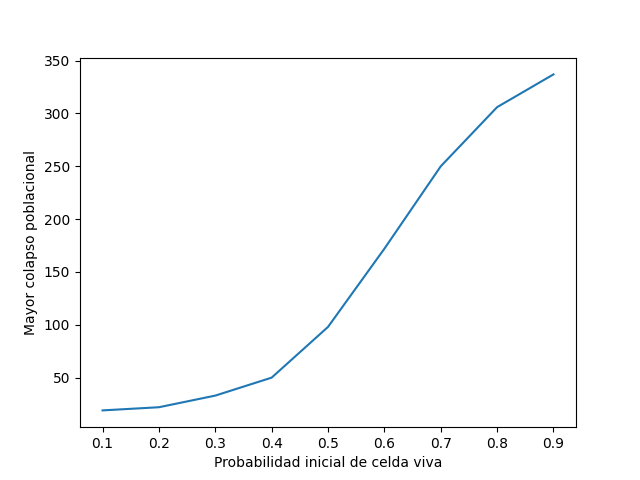
\includegraphics[width=\linewidth]{Figure_1.png}
\caption{Ejemplo de la asignación de edades con distribución exponencial.}
\end{figure}

\begin{figure}
\label{fig:F2}
\centering
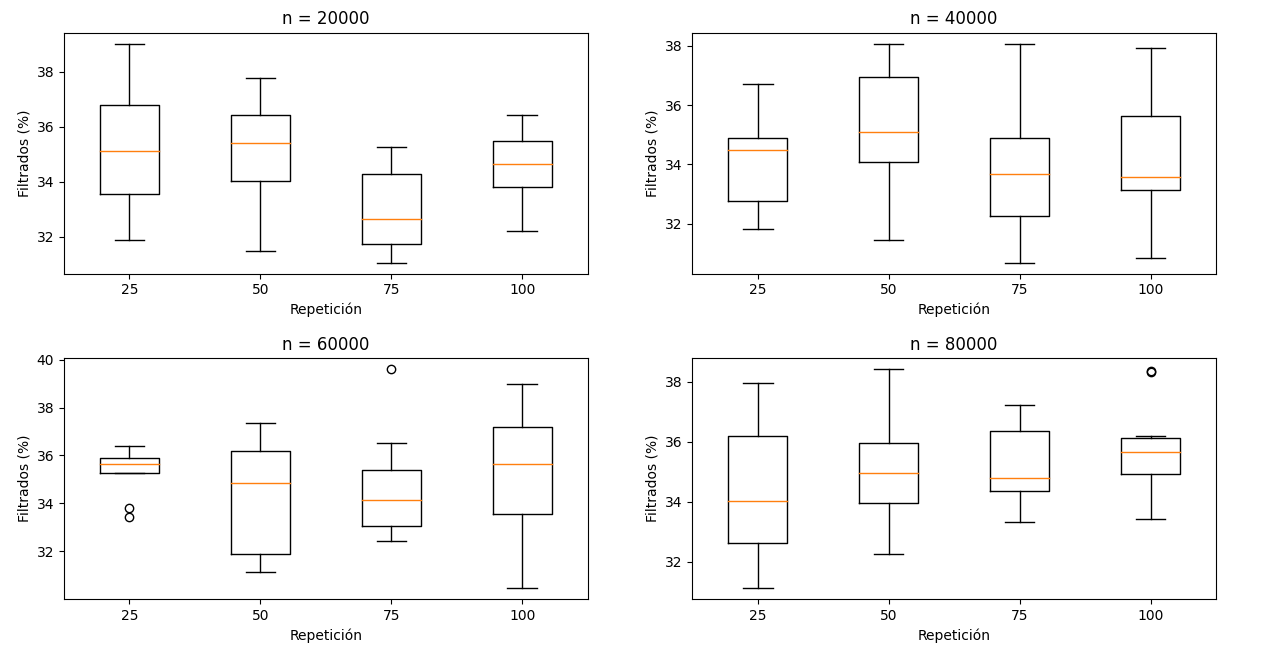
\includegraphics[width=\linewidth]{Figure_2.png}
\caption{Función de la probabilidad de muerte (pm).}
\end{figure}
 

Para demostrar los efectos de los super esparcidores se cuenta con el espacio ya conocido en la actividad \cite{VO-P6} en donde es visible cada uno de los agentes y su movimiento, pero esta vez estará dividido en 4 cuadrantes diferentes contando cada uno de ellos con el mismo número de agentes. La división de estos cuadrantes representa areas aisladas entre sí impidiendo el contagio entre agentes de diferente cuadrante, esto puede verse representado en la Figura \ref{fig:F1}. Una vez teniendo esta primera instancia en donde tenemos un solo infectado en uno de los cuadrantes podemos correr la simulación para observar el comportamiento que tiene el aislamiento de los agentes en los cuadrantes, esto puede verse representado en la Figura \ref{fig:F2}. Una vez observada la Figura \ref{fig:F2} podemos determinar que el efecto causado por el aislamiento es; impedir la propagación de la infección entre los agentes de diferentes cuadrantes. Ahora se realizará la misma simulación, sin embargo serán agregados los super esparcidores los cuales tendrán la característica de poder moverse entre cuadrantes. El inicio de esta simulación podrá observarse en la Figura \ref{fig:F5}, mientras el final de la simulación podrá observarse en la Figura  \ref{fig:F6}.

\begin{figure}
\label{fig:F3}
\centering
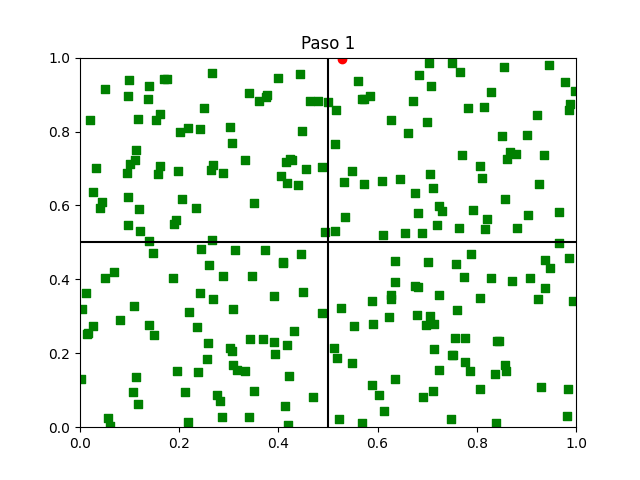
\includegraphics[width=\linewidth]{Figure_3.png}
\caption{Simulación con 4 cuadrantes sin super esparcidores, paso 1.}
\end{figure}



\begin{figure}
\label{fig:F4}
\centering
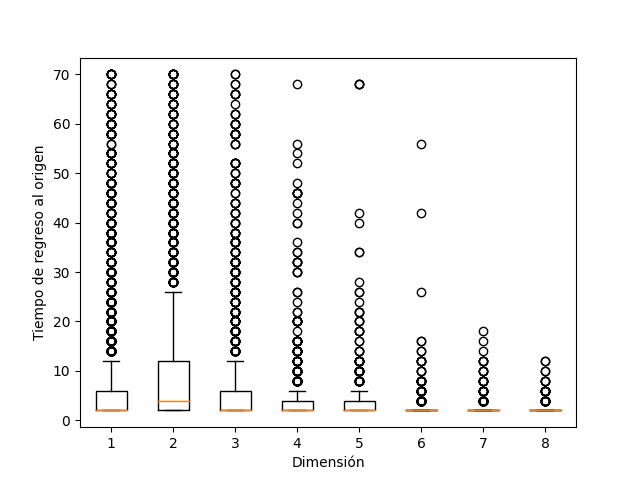
\includegraphics[width=\linewidth]{Figure_4.png}
\caption{Final de la simulación con 4 cuadrantes sin super esparcidores, paso 200.}
\end{figure}


\begin{figure}
\label{fig:F5}
\centering
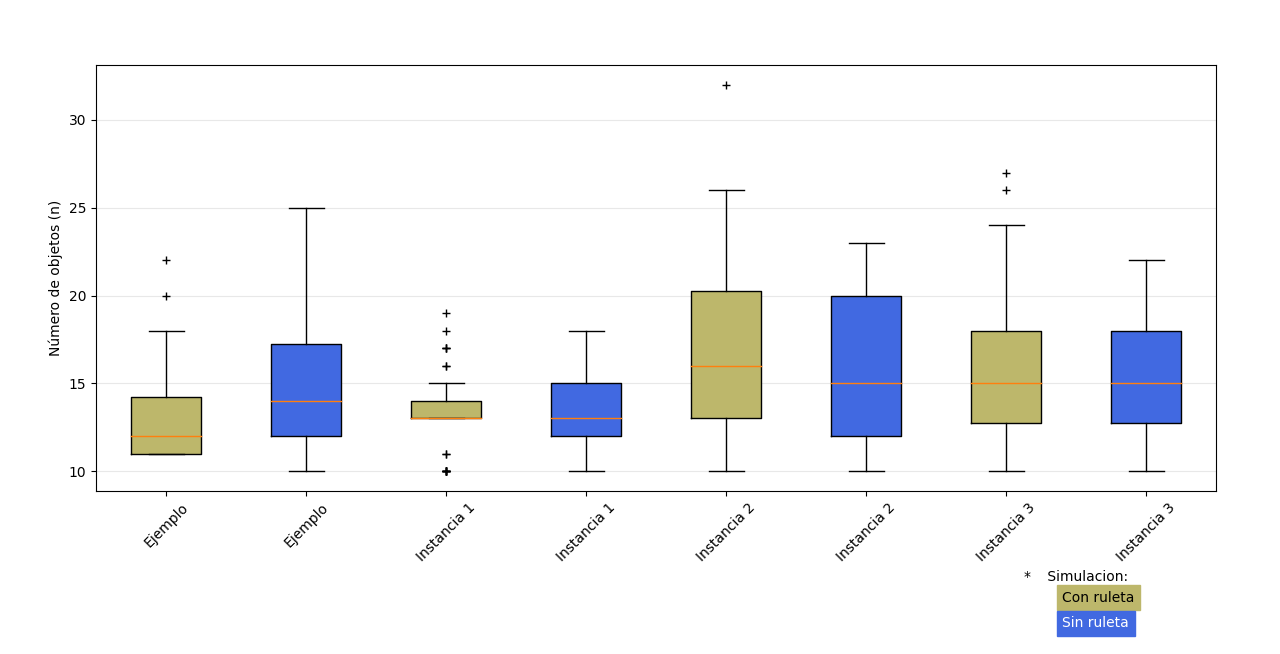
\includegraphics[width=\linewidth]{Figure_5.png}
\caption{Simulación con 4 cuadrantes con super esparcidores, paso 1.}
\end{figure}

\begin{figure}
\label{fig:F6}
\centering
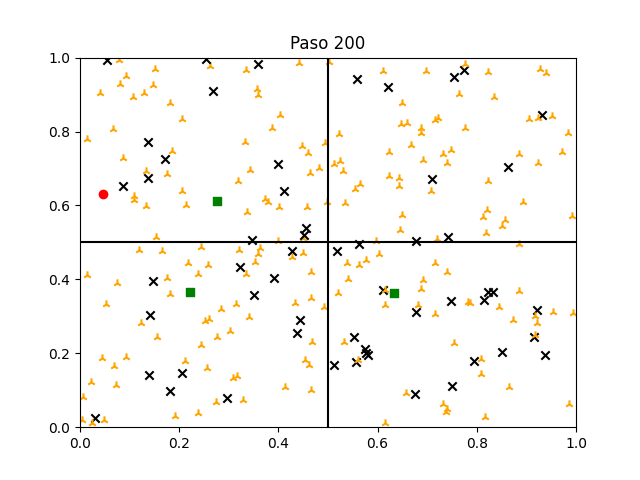
\includegraphics[width=\linewidth]{Figure_6.png}
\caption{Final de la simulación con 4 cuadrantes con super-esparcidores, paso 200.}
\end{figure}



Una vez terminada la simulación con los super esparcidores podemos observar como el aislamiento a sido corrompido y todos los cuadrantes han sido infectados. Para tener una mayor claridad del transcurso de ambas simulaciones se tienen la Figura \ref{fig:F7} y \ref{fig:F8}.

\begin{figure}
\label{fig:F7}
\centering
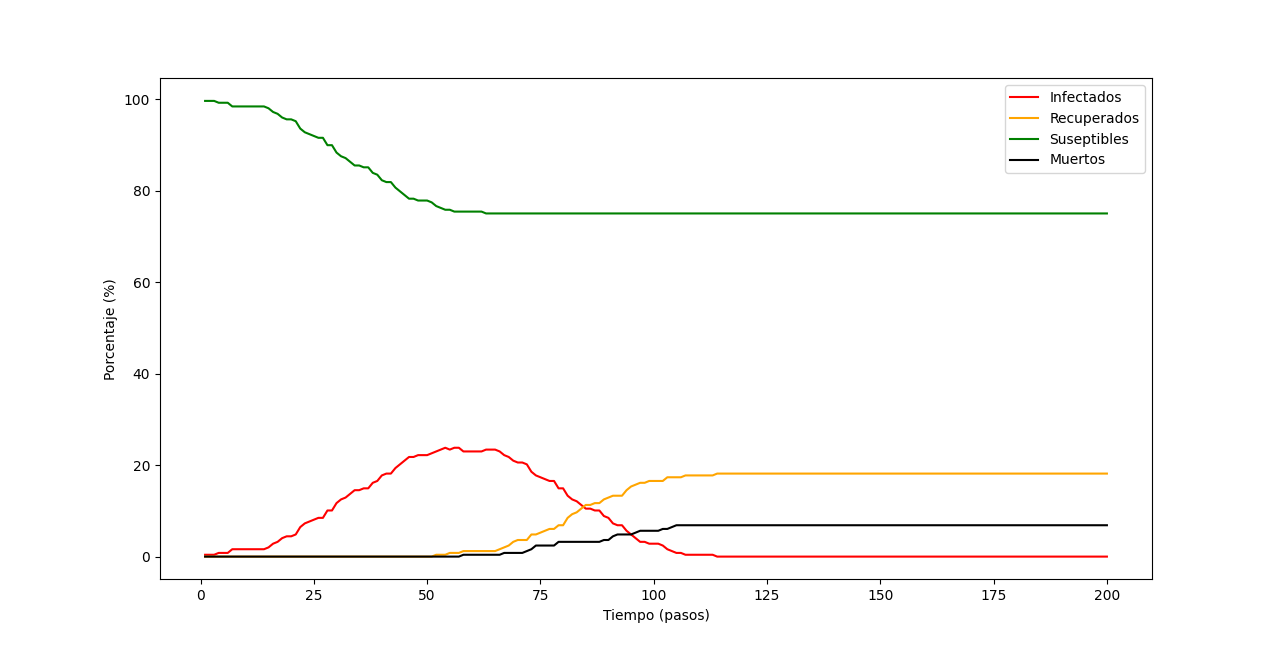
\includegraphics[width=\linewidth]{Figure_7.png}
\caption{Estadísticas de la simulación con 4 cuadrantes sin super esparcidores.}
\end{figure}

\begin{figure}
\label{fig:F8}
\centering
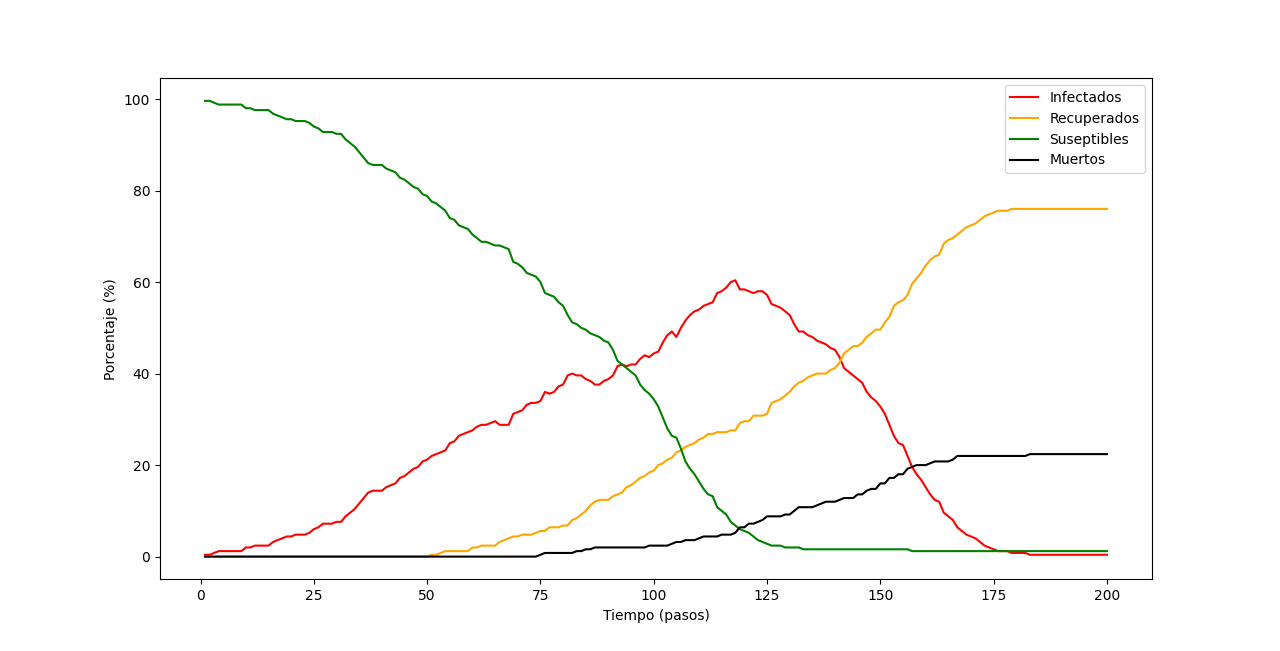
\includegraphics[width=\linewidth]{Figure_8.png}
\caption{Estadísticas de la simulación con 4 cuadrantes con super esparcidores.}
\end{figure}

Una vez comprobado los efectos que tienen los super esparcidores en la simulación, el objetivo es encontrar el porcentaje mínimo para detener en cierta medida la epidemia. Por lo tanto se genera una probabilidad de vacuna \texttt{(pv)} por lo que al inicio de generar la instancia de cada agente, estos podrán desde un inicio contar con el estatus Recuperado sin la necesidad de haber sido contagiado. Esta probabilidad solo será aplicado para los super esparcidores. Para comprobar el efecto de la probabilidad de vacuna \texttt{(pv)} sobre la dinámica de la epidemia se realizaran simulaciones con \texttt{(pv)} diferentes, con un rango desde 0 hasta 1. Los resultados de esta simulación se reflejan el la Figura \ref{fig:F9}.


\begin{figure}
\label{fig:F9}
\centering
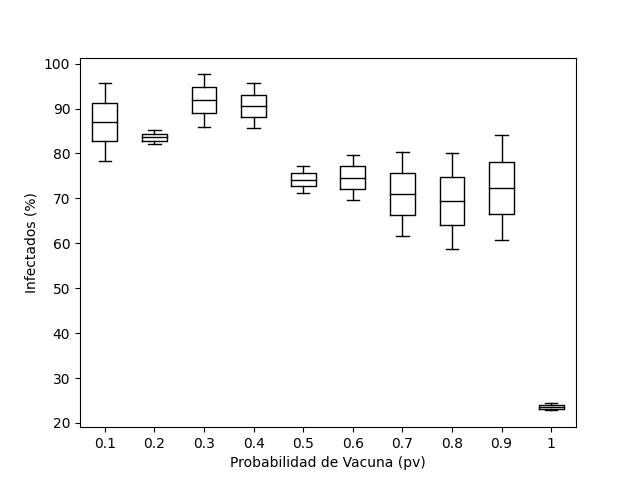
\includegraphics[width=\linewidth]{Figure_9.png}
\caption{Resultados de la simulación con diferentes valores de (pv) a 3 repeticiones.}
\end{figure} 

Con base en los resultados de la Figura \ref{fig:F9} podemos afirmar que desde la probabilidad de vacuna \texttt{(pv)} 0.1 hasta 0.4 la pandemia no a sido controlada ya que se tienen porcentajes de infectados mayores al 80\% lo que significa que todos los cuadrantes fueron infectados. Se tiene el Cuadro \ref{E.cuadro} para las equivalencias de porcentaje de infectados a cuadrantes infectados. Observando la probabilidad de vacuna 0.5 hasta 0.9 observamos que el porcentaje de infectados es menor, por lo tanto se realizan nuevas simulaciones pero esta vez con rango desde 0.8 hasta 0.85 y esta vez a 10 repeticiones cada \texttt(pv).

\begin{table}
\centering
\label{E.cuadro}
\caption{Equivalencia de porcentaje de infectados a cuadrantes infectados.}
\begin{tabular}{|c|c|}
\hline 
 Infectado (\%) & Cuadrantes (\#) \\ 
\hline 
20 & 1 \\ 
\hline 
40 & 2 \\ 
\hline 
60 & 3 \\ 
\hline 
80 & 4 \\ 
\hline 
\end{tabular} 
\end{table}


\begin{figure}
\label{fig:F10}
\centering
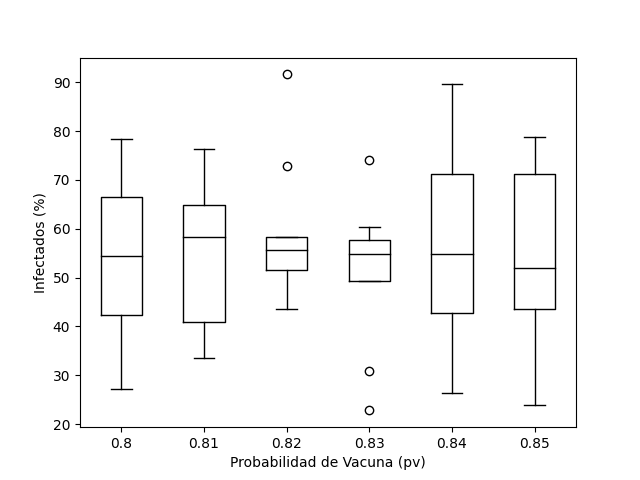
\includegraphics[width=\linewidth]{Figure_10.png}
\caption{Resultados de la simulación con diferentes valores de (pv) a 10 repeticiones.}
\end{figure} 

%----------------------------------------------------------------------------------------------


\section{Conclusiones}

Al obtener los resultados de la Figura \ref{fig:F10} lo que podemos ver es una muy clara similitud en las simulaciones, sin embargo al comparar los resultados de Figura \ref{fig:F9} específicamente los del la probabilidad 0.8, tenemos que su mediana es de aproximandamente el 70\% de infectados mientras que en los datos de Figura \ref{fig:F10} su mediana es de aproximandamente el 55\%. Recordando que en una simulación se realizaron 3 repeticiones y en la otra 10 repeticiones, esto nos indica que para una mejor definición de resultados se necesitaría una mayor cantidad de repeticiones, sin embargo al no contar esta simulación con multiprocesamiento el tiempo de simulación es considerable, ya que el tiempo de simulación depende de la cantidad de agentes pero mayor mente de la cantidad de agentes infectados. Por ese motivo para Figura \ref{fig:F9} solo se le ha permitido tener 3 repeticiones mientras que Figura \ref{fig:F10} se ha permitido tener 10 repeticiones, y aún así el tiempo de la Figura \ref{fig:F9} es mayor. \\

Por otra parte, con los datos obtenidos de la Figura \ref{fig:F10}, podemos observar que la pandemia solo llega a infectar a aproximadamente el 55\% de la población, por lo tanto podemos decir que vacunando desde aproximadamente el 16\% de la población total es posible controlar la epidemia, sin embargo este 16\% tendría que ser específicamente los super esparcidores, o como se demuestra en la Figura \ref{fig:F9} vacunar al 100\% super esparcidores. \\

Como trabajo futuro sería de suma importancia añadir multiprocesamiento a este código, ya que gran parte de su limitante reside en el tiempo que tarda en realizar completamente una simulación, por lo que al aplicar repeticiones es inviable el tiempo que esta llega a tardar, esto sin tomar en cuenta que la cantidad de agentes en esta simulación es relativamente baja (250 agentes). Por otra parte una mejora considerable al intentar simular el virus SARS-CoV-2 sería agregar un tiempo de inmunidad en el que una vez pasados cierto tiempo los agentes recuperados vuelvan a ser susceptibles y por lo tanto pueden volver a ser contagiados. De ser nuevamente contagiados se podría tener 3 o hasta 4 funciones diferentes de la probabilidad de muerte, en el que dependiendo de la cantidad de veces que haz sido infectado le corresponde una función, tomando en cuenta que la función será cada vez mas severa. De esta forma podríamos observar verdaderas fluctuaciones en la simulación pudiendo llegar a la extinción.  
%----------------------------------------------------------------------------------------------


\bibliographystyle{plainnat}
\bibliography{P.ref.bib}




\end{document}